
\chapter{Introduction}


% \section{Contextualization}


    % [IA-GEN NA INDUSTRIA] 
    In the dynamic changing of the oil and gas (O\&G) industry, digital transformation has emerged as a key element to achieve operational efficiency, sustainability, and competitiveness. 
    At the forefront of this transformation are Large Language Models (LLMs), which have the potential to process unstructured queries, map out alternatives, and advise users on possible actions \cite{Kar2023}. 
    We also note the advantage of increased engagement, cooperation, accessibility, and ultimately profitability. 
    These models redefine paradigms in knowledge management and information retrieval and impact a variety of other areas \cite{Eckroth2023}, making it crucial to adopt these technologies to remain competitive.    
    
    % [ESTUDO AUMENTO PRODUTIVIDADE] 
    A study conducted by \cite{Dellacqua2023}, in collaboration with the Boston Consulting Group demonstrates that in knowledge-intensive tasks, consultants equipped with access to LLMs like GPT-4 not only completed tasks more efficiently (25.1\% more quickly on average) but also with substantially higher quality, achieving results more than 40\% better compared to those without AI assistance \cite{Dellacqua2023}. Increase in productivity of knowledge workers was 12\% on average.    
    A major oil company spent in 2023 \$2.8B with employee compensation. A potential increase of 12\% in knowledge workers productivity, given they represent 60\% of all employee, could represent \$204M annual savings in this scenario.     
    % [AUMENTO DO PIB DEVIDO A GEN AI] 
    Broader economic indicators predict significant transformations due to generative AI (Gen-AI) across various industries.
    A report from Goldman Sachs \cite{Hatzius2023} highlights that Gen-AI is poised to increase global GDP by nearly 7\%, increasing productivity growth by 1.5 percentage points over the next decade. 
    This economic uplift is expected due to AI's ability to automate complex workflows and create new business opportunities, significantly impacting employment and productivity sectors worldwide.
            
    % [PROBLEMA DE DADOS NA INDUSTRIA EM GERAL] 
    Expanding on the broader discussion on data utilization within organizations, an important issue is the challenge of extracting relevant information from extensive databases \cite{Singh2023}. 
    Initially, the challenge of knowing, finding, and accessing data poses a significant obstacle to decision-making processes. Collaborators at O\&G companies often face the intensive task of manually searching large data repositories to find useful information.
    
    % [PROBLEMA DE DADOS NO O\&G] 
    Focusing specifically on the activities of drilling and completion of offshore and onshore wells, a major challenge lies in the inherently complex and technical nature of the data involved, which can be from various types: operations, projects, technologies, supply chains, and others. 
    Inefficiency in leveraging large volumes of unstructured data worsens these challenges, as observed by \cite{Singh2023}. A significant amount of the data generated and collected in this sector is unstructured, ranging from text reports and emails to images and videos of exploration and production activities. 
    Examples include hundreds of daily operational reports from drilling rigs, well execution projects, nonproductive time (NPT) reports, and operational lessons learned documents, as illustrated in Figure \ref{fig:report_example}. 
    As a result, valuable information can remain untapped, and the potential to find insights, informed decision-making and innovation is significantly compromised.
    \cite{Singh2023} showcases the capabilities and potential of Generative AI-enabled chatbots for the O\&G sector, particularly in enhancing drilling and production analytics to achieve better business outcomes. The author concludes that companies that adopt these technologies in the coming years will see clear advantages.     
    
    \begin{figure}[t]
        \centering
        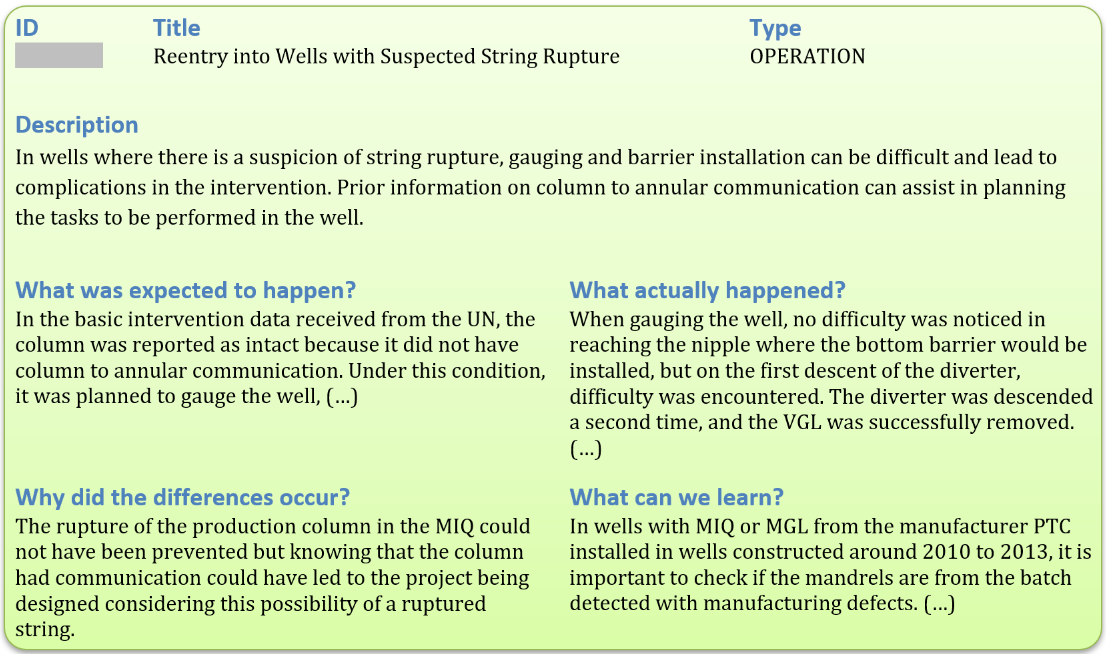
\includegraphics[width=1\textwidth]{images/report_example.png}
        \caption{Sample of drilling \& completion learned lesson partial document. (translated from Portuguese)}
        \label{fig:report_example}
    \end{figure}           
    
    However, the deployment of such technologies presents limitations and introduces challenges, including biased data, hallucinations, lack of explainability, and logical reasoning errors, among others \cite{Hadi2023}, which require a balanced approach to harness their potential in a responsible manner.    
    Although previous research has focused mainly on the broader applications of AI in industry, the novelty of our research lies in its original examination of the specific challenges and solutions presented by the complex, technical and unstructured data inherent in O\&G operations. By comparing single- and multi-agent systems, this study fills a knowledge gap, providing empirical insights into the effectiveness of different Gen-AI architectures in a domain where such studies are scarce. 
    
    The adoption of these technologies by a major oil company underscores their potential to revolutionize data analysis and management, presenting an opportunity for deeper exploration and application.


\section{Objectives}

    This research directly addresses challenges faced by major oil companies. By investigating the comparative advantages and limitations of various Gen-AI architectures, including single and multi-agent systems, for Q\&A and Text-to-SQL tasks, this study aims to identify the most efficient and cost-effective solutions.
    The specific objectives of this research are to assess the suitability and effectiveness of multi-agent systems based on LLMs for complex, domain-specific tasks in well engineering, aiming to streamline information access and decision-making. 
    The study will compare single-agent and multi-agent AI systems in terms of their ability to address well engineering queries. Finally, it will map the potential obstacles and limitations associated with deploying Gen-AI applications.
            
    The insights gained from this research will directly contribute to O\&G companies strategic goals by improving access to well engineering information and automated data analysis tasks. 
    A comprehensive understanding of the challenges and limitations associated with Gen-AI will enable informed decisions about its adoption, maximizing the return on investment. 

    To achieve these objectives, this research was conducted through two distinct experimental phases. The first, carried out in 2024, focused on a foundational comparison between single and multi-agent architectures, revealing key insights into their performance, cost, and limitations such as hallucination and context interpretation. The rapid evolution of generative AI frameworks and models prompted a second, more advanced experiment in 2025. This second phase built upon the initial findings, also employing non-agentic workflows as baseline and a more rigorous, quantitative evaluation methodology to address the challenges identified in the first experiment and automated evaluation based on the concept commonly reffered to as "LLM-as-judge" (\cite{Gu2025}).

\section{Business Scope Delimitation}

    To contextualize the scope of this study, it is necessary to understand the life cycle of an oil field, which begins with Exploration and progresses to the Development of Production, followed by effective production, and culminates in decommissioning \cite{Badiru2016}. Gen-AI has the potential to impact each of these phases, but the focus of this work lies in the operations of the development and maintenance stages.
            
    Well construction is a highly specialized activity involving drilling and completion of wells for hydrocarbon extraction \cite{Thomas2004}. In this context, Gen-AI can be applied in various ways. For example, a chatbot could manage knowledge by answering queries about operations and well projects by retrieving information from the organization's databases. Additionally, LLM-based agents could be used in executive project review to ensure that drilling or completion operations comply with the organization's standards and adhere to best operational practices. Moreover, Gen-AI could perform inference in unstructured databases to extract specific information from text reports and obtain structured data. 
    
    This business scope emphasizes the importance of Gen-AI in the construction and maintenance of wells.

\section{Thesis Structure}

    ****SERÁ FEITO POR ÚLTIMO****
